% typ dokumentu,draft
\documentclass[12pt,twoside]{article}

% użycie pakietu , jak include
\usepackage{weiiszablon}

% autor pracy
\author{Krystian Olszowy}

% np. EF-123456, EN-654321, ..., Numer albumu
\studentID{EA-167582}

\title{Aplikacja na smartfony do sterowania telewizorem}
\titleEN{{Mobile application for controlling TV set}}


%%% wybierz rodzaj pracy wpisując jeden z poniższych numerów: ...
% 1 = inżynierska	% BSc
% 2 = magisterska	% MSc
% 3 = doktorska		% PhD
%%% na miejsce zera w linijce poniżej
\newcommand{\rodzajPracyNo}{1}


%%% promotor
\supervisor{dr inż. Jan Sadolewski}
%% przykład: dr hab. inż. Józef Nowak, prof. PRz

%%% promotor ze stopniami naukowymi po angielsku
\supervisorEN{Jan Sadolewski, PhD, Eng.}

\abstract{Treść streszczenia po polsku}
\abstractEN{Treść streszczenia po angielsku}

\keywords{pilot, BLE, IR, Flutter, aplikacja mobilna}
\keywordsEN{remote controller, BLE, IR, Flutter, mobile application}


\begin{document}

% strona tytułowa
\maketitle

\blankpage

% spis treści
\tableofcontents

\clearpage
\blankpage

\section{Wstęp}
\subsection{Telewizor i sposoby sterowania nim}
Współcześnie nie wyborażamy sobie domu, w którym nie ma telewizora. Telewizory, będące
centralnym elementem więszkości domostw, przekształciły się z tradycyjnych urządzeń
telewizyjnych w zaawansowane systemy multimedialne, oferujące nie tylko dostęp do programów telewizyjnych,
ale również do różnorodnych treści wideo, gier, czy nawet aplikacji internetowych.
Ich powszechność we współczesnym świecie, a także mnogość producentów i ich pomysłów
sprawiło, że wyodrębniło się wiele technologii i sposobów sterowania tymi urządzeniami.

W wielu gospodarstwach domowych znajduje się wciąż telewizor sterowany jedynie za pomocą podczerwieni i jest
to nadal najpopularniejszy sposób sterowania tymi urzadzeniami. Rozwiązania takie jak sterowanie poprzez WiFi, czy Bluetooth
mimo, że są już pewien czas na rynku jeszcze nie goszczą u wszystkich użytkowników, zazwyczaj z powodu ceny
nowego urządzenia multimedialnego lub zwykłego braku potrzeby wymiany telewizora. Czy jest jednak sposób aby
móc korzystać z wygody nowych rozwiązań komunikacji bezprzewodowej, mając urządzenie zdolne do sterowania
telewizorem zawsze w naszej kieszeni dla urządzeń telewizyjnych nie posiadających obsługi nowoczesnych technologii bezprzewodowych?

\subsection{Smartfon i jego powszechność}
W dynamicznie rozwijającym się świecie, smartfony stały się nieodłącznym elementem życia społecznego,
definiując nowy wymiar komunikacji, rozrywki i funkcji użytkowych.
W ciągu ostatnich kilku dekad, powszechność smartfonów osiągnęła niespotykany poziom,
stając się nie tylko przedmiotem codziennego użytku, lecz również nieodzownym
narzędziem wspierającym wszystkie aspekty naszego życia.

Obecnie smartfony są nie tylko urządzeniami komunikacyjnymi, ale także mobilnymi centrami multimedialnymi,
umożliwiającymi dostęp do rozmaitych treści, od filmów i muzyki, po aplikacje społecznościowe.
Ich interaktywne interfejsy i intuicyjne systemy operacyjne sprawiają, że stają się łatwe w obsłudze nawet dla osób starszych,
które powoli przekonują się do współczesnej wersji telefonów komórkowych.

Z uwagi na wyżej wymienione zalety samrtfonów naturalnym pomysłem wydaje się także użycie ich do
sterowania urządzeniami multimedialnymi, w tym także telewizorów. Właściwie wszystkie współczesne smartfony posiadają
wcześniej wspomniane nowoczesne technologie komunikacji bezprzewodowej jak WiFi i Bluetooth, jednak nie uświadczymy
zbyt często już w nich obsługi podczerwieni. Aby skomunikować więc przy ich pomocy smartfon
ze starszym telewizorem, powstaje potrzeba dołączenia pośrednika tłumaczącego interakcję
użytkownika z aplikacją mobilną na sygnały podczerwone, które zrozumie telewizor.

\subsection{Cel pracy}
Celem pracy jest zaproponowanie rozwiązania sterowania telewizorem z poziomu
smartfona dzięki aplikacji mobilnej, komunikującej się z systemem pośredniczącym opartym o płytkę , który to system ma być oparty o mikrokontroler wraz odpowiednimi komponentami, mający za zadanie wysyłać sygnały podczerwone do telewizora. System ma zapewniać możliwość programowania przycisków dzięki dedykowanemu ekranowi w aplikacji i
wyświetlania odebranego kodu sygnału podczerwonego na wyświetlaczu zintegrowanym z mikrokontrolerem.

\subsection{Zakres pracy}
Zakres pracy obejmuje omówienie podobnych dostępnych rozwiązań na rynku, budowę systemu z~mikrokontrolerem na płytce ESP32 razem z wymaganymi modułami i utworzenie jego oprogramowania sterującego ,~a także projekt i oprogramowanie aplikacji
mobilnej frameworka Flutter służącej jako interfejs pilota uniwersalnego do telewizora. W obszarze zagadnień pedejmowanych w pracy znajduje się także przedstawienie działania zaprojektowanej aplikacji współpracującej ze zbudowanym urządzeniem pośredniczącym oraz wskazanie potencjalnych możliwości rozbudowania systemu.

\subsection{Zawartość pracy [niezakończone]}
W rozdziale drugim  omówiono ogólnodostępne rozwiązania stanowiące aktualny stan wiedzy w zakresie zdalnego sterowania odbiornikiem telewizyjnym.

\clearpage
\section{Porównanie zaprojektowanego systemu z do\-stęp\-ny\-mi rozwiązaniami}
\subsection{Omówienie dostępnych rozwiązań}
Na rynku można znaleźć niezliczoną ilość pilotów uniwersalnych. Rożnią się one
ceną, obsługiwanymi funkcjonalnościami czy sposobami zasilania. Większość z nich zazwyczaj
wykorzystuje programowanie oparte na nasłuchiwaniu sygnałów, co dla niektórych użytkowników może stanowić
wyzwanie ze względu na uciążliwą obsługę procesu, wymagającą ciągłej modyfikacji odbieranego
sygnału podczerwonego dla każdego przycisku. Cena rzędu jedynie kilku czy kilkunastu złotych
już na polskim rynku jednak kusi potencjalnych nabywców pomimo wątpliwej jakości wykonania. Przykładem
takiego pilota uniwersalnego może być urządzenie Interlook L336\cite{cheapController}.

Więksi producenci oferują również piloty uniwersalne z predefinowanymi sygnałami dla przycisków jednak
prawie zawsze są to modele właśnie tego producenta. Oczom nie umyka tażke wyższa cena takich
rozwiązań argumentowana zazwyczaj prestiżem marki i jakością wykonania. Takie rozwiązanie znaleźć
możemy na przykład w modelu Philips SRP4030/10\cite{expensiveController}.

Dostępne są jednak także rozbudowane aplikacje z dedykowanymi urządzeniami wysyłającymi sygnały podczerwone łączące się ze smartfonem poprzez WiFi. Znajdujemy już w nich wiele z pożądanych cech w pilocie uniwersalnym jak: niska cena względem oferowanych możliwości, możliwość otrzymania predefiniowanych modeli telewizorów czy edycję nie wymagającą posiadania oryginalnego pilota do sterowanego urządzenia. Przykładowym dostępnym rozwiązaniem tego typu jest urządzenie Smart IR Remote Crabtree\cite{appController}.
\subsection{Zestawienie z autorskim projektem}
{Wymienione wcześniej urządzenia mają swoje zastosowania jedank nie wystrzegają się wad.
   Wiele z nich wymaga zasilania bateryjnego co jest szkodliwe dla środowiska, o które szczególnie
   stara się dbać społeczeństwo w dzisiejszych czasach. Posiadają one często mozolne i łatwe w niepoprawnym użyciu
   programowanie. Dostęp do tworzenia własnych
   zestawów przycisków jest w nich nierzadko trudny, czasem niemożliwy, a użycie często wymaga
   przeskakiwania po liście i sprawdzeniu czy telewizor reaguje na predefiniowane przyciski. Urządzenia nieposiadające tych wad czyli aplikacje z dedykowaną stacją wysyłającą sterowanie do urządzeń domowych łączą się jednak poprzez WiFi ze smartfonem przez co pobiera ono więcej energii niż inne rozwiązania oraz wymaga podłączenia tego urządzenia do sieci użytkownika co zmniejsza jej bezpieczeństwo.

   Autorskie rozwiązanie systemu służacego za pilota do telewizora stara się rozwiązać przedstawione problemy. Bateria czy akumulator możliwe
   są do używania z urządzeniem wysyłającym sygnały podczerwone, jednak z powodzeniem zasilanie może i powinno odbywać się przez
   kabel microUSB, dzięki czemu nie zwiększany jest popyt na szkodliwe dla środowiska baterie. Programowanie przycisków
   odbywa się przez podanie kodów IR w odpowiednich polach, które sprawdzają czy dane w nich zawarte są poprawne, dzięki czemu użytkownik ma bezpośredni i przejrzysty dostęp do swoich ustawień pilota. Utworzony przez użytkownika lub predefiniowany
   model telewizora wybierany jest z listy, którą można łatwo przeglądać i rozbudować. Sama aplikacja posiada kontrolę błędów konfiguracji oraz sieci
   i jest intuicyjna dla użytkownika już podczas pierwszego uruchomienia. Komunikacja ze smartfonem odbywa się za pomocą protokołu BLE co ogranicza zużycie energii. Zauważając, że z urządzenia pośredniczącego może korzystać wiele osób jednocześnie w większej skali jest to tańsze rozwiązanie niż piloty
   uniwersalne. Łatwość obsługi i przejrzystość interfejsu aplikacji jest atutem zwłaszcza dla osób starszych, nieobytych z technologią.
}
\clearpage
\section{Przedstawienie wykorzystanych technologii}
\subsection{Platforma ESP32}
ESP32 jest układem typu SoC (ang. System-on-a-chip) produkowanym przez chińską firmę Espressif Systems,
wyposażony jest najczęściej w dwurdzeniowy procesor Xtensa LX6 o taktowaniu 240 MHz\cite{esp32Datasheet}. Przez hobbystów w większości przypadków używany jest będą osadzonym na płytce deweloperskiej różnych producentów co przyspiesza projektowanie i prototypowanie rzeczywistego systemu. Na runku znajduje sie niezliczona ilość różnych wersji płytek deweloperskich przez co dopasowanie
jej do własnych potrzeb jest znacznie łatwiejsze niż rozważając inne rozwiązania. Przykładem takiej płytki, która zarazem została użyta w projekcie jest DOIT DevKit V1\cite{doitDevKitV1}.Na rysunku \ref*{Fig:devkitScheme} przedstawiono poglądowy shemat wyprowadzeń tej płytki deweloperskiej.

\begin{figure}[ht]
   \centering
   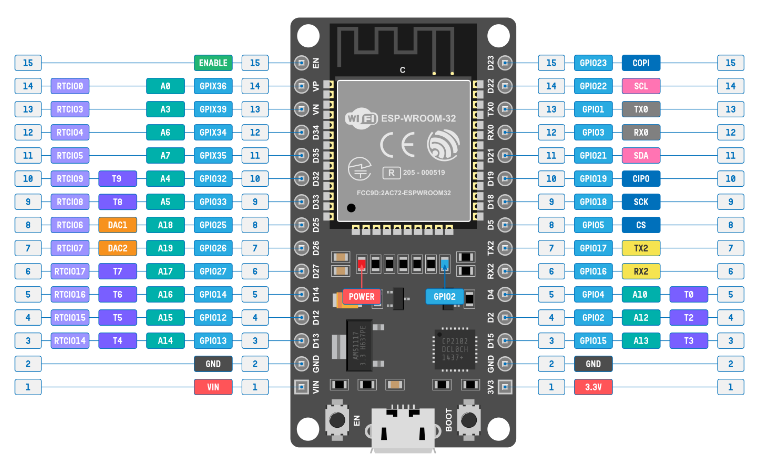
\includegraphics[width=13cm]{images/doit_devkit_v1.png}
   \caption{Schemat wyprowadzeń płytki DOIT DevKit V1 \cite{doitDevKitV1}}
   \label{Fig:devkitScheme}
\end{figure}

Jednym z kluczowych atutów ESP32 jest wbudowane wsparcie dla Wi-Fi(802.11 b/g/n) i Bluetooth(klasyczny 4.2 i BLE),
co umożliwia łatwe połączenie z siecią bezprzewodową oraz sprawną komunikację między urządzeniami zewnętrznymi.
Duża licz\-ba portów wejścia/wyjścia czyni go idealnym do obsługi wielu czujników, akscesoriów i modułów. Układ zawiera także
zintegrowany konwerter analogowo-cyfrowy (ADC) umożliwia precyzyjny pomiar sygnałów analogowych. System zawiera wiele innych możliwości, ale najważniejsze funkcjonalości i charakterystyczne cechy firma Espressif zebrała na digramie który znalazł się na rysunku \ref*{Fig:functionalDiagram}.

\begin{figure}[ht]
   \centering
   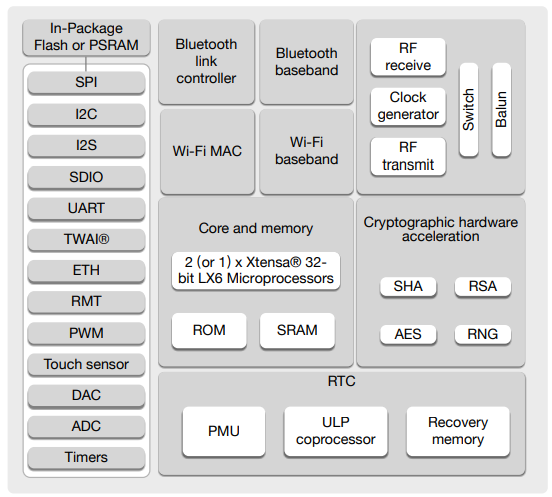
\includegraphics[width=12cm]{images/esp32_functional_diagram.png}
   \caption{Diagram funkcjonalności zaczerpnięty z dokumentacji techniczej ESP32\cite{esp32Datasheet}}
   \label{Fig:functionalDiagram}
\end{figure}

ESP32 został także zoptymalizowany pod kątem efektywnego zużycia energii, co sprawia, że jest bardzo dobrym
wyborem dla aplikacji zasilanych bateryjnie lub kiedy zwyczajnie ważny jest niski pobór prądu. Jego wszechstronność objawia
się obsługą przeróżnych protokołów komunikacji przewodowej,
takich jak SPI, I2C, UART, co ułatwia integrację z zewnętrznymi modułami i systemami.

Warto podkreślić, że ESP32 cieszy się uznaniem wśród społeczności deweloperów, co przekłada się na dostęp
do obszernej dokumentacji oraz wsparcie online. Programowalność w języku Arduino oraz możliwość korzystania
z MicroPython dodatkowo zwiększają elastyczność platformy, umożliwiając dostosowanie do indywidualnych potrzeb projektu.
Nieocenione są także biblioteki i moduły tworzone przez społeczność i udostępniane w formie otwartoźródłowej.
\subsection{Język programowania C++}
Język C++ jest językiem programowania, który swoje zastosowanie znalazł w wielu dziedzinach gdzie ceni się wydajność rozwiązania. Mimo tego że powstał w latach 80-ątych na podstawie języka C, jego najnowsze wersje zdecydowanie można zaliczyć do nowoczesnych języków programowania.

Język ten jest kompilowany oraz sostuje silne typowanie statyczne, dzięki czemu wykrywanie błędów na etapie tworzenia kodu jest znacznie łatwiejsze niż w przypadku innych podejść tworzenia programu wynikowego. Charakteryzuje się on także niskopoziomowym dostępem do pamięci jak i możliwością jej dynamicznej alokacji w trakcie trwania programu co zapewnia elastyczność implementacji i wysoką wydajność. C++ daje także możliwość korzystania z specyfikatora inline, który powoduje, że kompilator kopiuje kod funkcji w zadane miejsce zamiast umiesczać tam wkaźnik wskaźnik do niej. Przekłada się to na minimalizację narzutu czasowego związanego z wywołaniami bloków funkcyjnych. Język ten umożliwia także stosowanie obiektowego podejścia do projektowania oprogramowania, co z kolei sprzyja modularności rozwiązania i łatwości utrzymania kodu.\cite{cppBjarne}

Wydajność i możliwość niskopoziomowej kotroli zasobów urządzenia powoduje, że język tn jest  najczęściej używany do programowania skomplikownych gier
komputerowych, protokołów komunikacyjnych oraz systemów wbudowanych. Przez jego popularność dla systemów wbudowanych, powstało wiele współracujacych z nim frameworków i bibliotek do obsługi rozmaitych mikrokontrolerów. Dzięki temu wybierając C++ jako język utworzenia oprogramowania systemu wbudowanego zyskuje się bardzo dużą kontrolę nad sprzętem oraz elastyczność w doborze narzędzi deweloperskich.

\subsection{Framework Arduino}
Framework Arduino\cite{arduinoIntroduction} to otwarte oprogramowanie, które umożliwia łatwe tworzenie aplikacji dla mikrokontrolerów zgodnych z Arduino.
Bazuje na języku programowania C++ oraz wykorzystuje uproszczoną warstwę abstrakcji, co sprawia, że
jest przyjazny dla początkujących, jednocześnie oferując zaawansowane funkcje dla doświadczonych programistów.

Framework oferuje prostą obsługę wejścia/wyjścia (I/O), dzięki czemu integracja z czujnikami, przekaźnikami, i wieloma innymi modułami jest błyskawiczna i intuicyjna. Ponadto, framework zapewnia prosty sposób dostęp do interfejsów komunikacyjnych,
takich jak UART, SPI czy I2C. Ważną częścią frameworka Arduino są też przyjazne w użyciu biblioteki tworzone także przez użytkowników, przez co niemal zawsze znajdzie się kod obsługujący żądaną funkcjonalność. Obejmują one obszar komunikacji bezprzewodowej, obsługi czujników, sterowania silnikami, czy obsługi ekranów LCD lub OLED. Każde z nich są regularnie poprawiane przez firmę lub społeczność dzięki czemu oprogramowanie staje się szybko aktualne i wspiera nowo dodane urządzenia i narzędzia.
\subsection{Komunikacja za pomocą podczerwieni}
Komunikacja przez podczerwień (IR - Infra-Red) to forma przesyłania danych, wykorzystująca fale elektromagnetyczne
o niższej częstotliwości niż światło widzialne. Fale podczerwone znajdują się w zakresie elektromagnetycznym
poniżej czerwonego końca widma światła widzialnego, typowo w zakresie od 300 GHz do 400 THz. Te fale są
niewidoczne dla ludzkiego oka, ale mogą być wykrywane i generowane przez diody. Typowo
wysyłając sygnał według konkretnego protokołu najpierw moduluje się go według określonego kodu liczbowego.
Modulacja może obejmować zmianę amplitudy, częstotliwości lub fazy fali podczerwonej. Gdy sygnał dociera do odbiornika
(zazwycza zasięg wynosi do 10m), odbiornik wyposważony także w diodę interpretuje odebrany sygnał, przeprowadzając proces demodulacji, do kodu
liczbowego. Z tak wysłanej informacji może teraz skorzystać urządzenie odbierające i podjąć na jej podstawie działania.

W standardzie NEC, czyli najpopularniejszym sposobie przesyłania sygnałów do urządzeń RTV, zastosowana jest modulacja częstotliwośći. Każda wiadomość w tym typie komunikacji rozpoczyna się od stosunkowo długiego stanu wysokiego natężenia światła trwającego 9 ms po czym następuje 4,5 ms przerwy sygnalizując rozpoczęcie nadawania. Chcąc teraz wysłać logiczną ,,1'' , należy wygenerować stan wysoki natężenia światła podczerwonego na 562.5µs i po nim odczekać 562.5µs. Logiczne ,,0'' wysyłane jest przez taki sam zabieg, jednak z przerwą po stanie wysokim wynoszącą 1.6875 ms. Aby bit został odczytany przez odbiornik każda przerwa musi być zakończona następnym stanem wysokim natężenia fali światła, dlatego kiedy kończona jest transmisja, po ostatniej przerwie generowany jest dodatkowy puls długości 562.5µs, aby odbiornik mógł odczytać długość przerwy ostatniego bitu. Wykres ilustrujący elementarna generację sygnału w tym standardzie przedstawia rysunek \ref*{Fig:necOnesZerosFigure}.
\begin{figure}[ht]
   \centering
   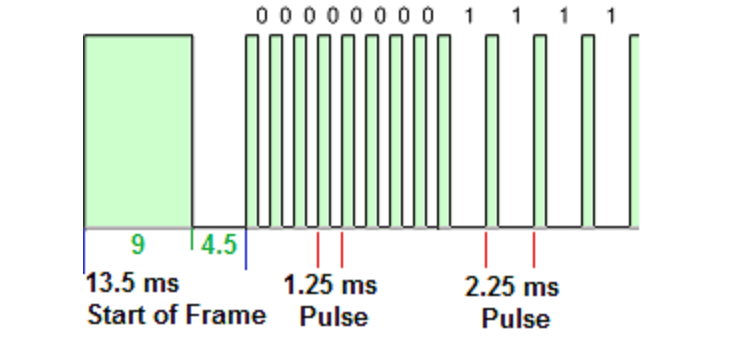
\includegraphics[width=8cm]{images/necOnesAndZeros.png}
   \caption{Wykres elementarnej modulacji sygnału standardu NEC\cite{necIR}}
   \label{Fig:necOnesZerosFigure}
\end{figure}

Aby wysłać pełne rządanie, które może być interpretowane przez odbiornik, trzeba wysłać informację opatrzoną w pewną strukturę. Najpierw wysyłany jest sygnał rozpoczęcia nadawania. Następnie wysyłany jest 8 bitowy adres urządzenia odbierającego sygnał i kolejno jego negacja bitowa. W takim sam sposób wysyłane jest 8 bitów danych i ich negacja bitowa. Tak zbudowana pojedyncza ramka danych potrzebuje zawsze 67,5 ms aby zostać wysłana niezależnie od danych i adresu dzięki negacji bitowej obu tych danych. Przykładowe wysłanie danej 0xAD do urządzenia o adresie 0xFF przedstawione zostało na wykresie \ref*{Fig:necFrame}.

\begin{figure}[ht]
   \centering
   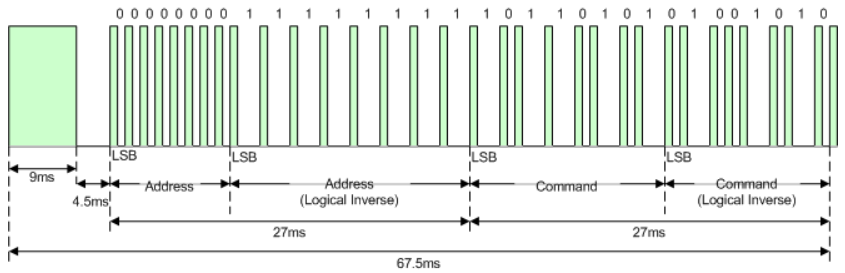
\includegraphics[width=13cm]{images/necFrame.png}
   \caption{Przykładowa modulacja sygnału pełnej wiadomości standardu NEC\cite{necIR}}
   \label{Fig:necFrame}
\end{figure}

\subsection{System operacyjny Android}
System Android, rozwijany przez firmę Google, stanowi środowisko operacyjne oparte na otwartym kodzie źródłowym,
co przyczynia się do jego wyjątkowej elastyczności i dostosowywalności do różnych urządzeń mobilnych, głównie
smartfonów i tabletów, ale z powodzeniem stosowany jest także w innych urządzeniach przenośnych.
Otwartość kodu umożliwia deweloperom z całego świata dostosowywanie systemu do specyficznych
potrzeb. Istotną cechą Androida jest także jego wszechstronność, manifestująca się w szerokiej gamie dostępnych
urządzeń posiadających zainstalowany ten system operacyjny.
Instalowany jest na urządzeniach z wszystkich przedziałów cenowych, umożliwiając
programistom tworzenie aplikacji dostępnych dla każdej z grup odbiorców. Sklep Google Play, jako główne źródło
aplikacji, gier, multimediów i innych treści, stanowi istotny element ekosystemu Androida. Ponadto, integracja
z usługami Google, takimi jak Gmail, Google Drive, Google Maps i wielu innych sprawia, że można niemal każdą czynnoś wykonać przy pomocy dedykowanej aplikacji firmy Google. Względną jednolitość tego środowiska pomimo takiej gamy obsługiwanych urządzń sprawia, że dla programistów stanowi ono atrakcyjne pole do
rozwoju i tworzenia innowacyjnych rozwiązań, z uwagi na szeroką bazę użytkowników oraz dynamiczny rynek aplikacji mobilnych. Nie jest dziwne więc, że urządzenia z Androidem posiadało 69,74\% wszytskich użytkowników urzadzeń mobilnych i był on najczęściej używanym systemem operacyjnym w 2022 roku\cite{androidStats}.
\subsection{Język programowania Dart}
Dart to język programowania stworzony przez Google, zaprojektowany z myślą o tworzeniu wydajnych, skalowalnych i nowoczesnych aplikacji. Jego głównym zastosowaniem jest budowa interaktywnych stron internetowych oraz aplikacji mobilnych przy użyciu zestawu narządzi Flutter.

Język ten charakteryzuje się statycznym typowaniem, co oznacza, że typy zmiennych są sprawdzane w trakcie budowania aplikacji, co może pomóc w wykrywaniu błędów przed uruchomieniem programu. Dart wspiera również programowanie obiektowe.

Jedną z ważnych cech Darta jest również jego zdolność do wykonywania kodu zarówno w trybie just-in-time (JIT),jak i ahead-of-time (AOT). Tryb JIT umożliwia szybkie rozwijanie i testowanie aplikacji, podczas gdy tryb AOT pozwala na kompilację
kodu źródłowego do natywnego kodu maszynowego, co przyspiesza wydajność aplikacji podczas działania. Dart oferuje także mechanizmy asynchroniczne, co jest istotne w programowaniu współbieżnym i obsłudze operacji wejścia/wyjścia bez blokowania głównego wątku.\cite{dartInfo}

W kontekście frameworka Flutter, język ten staje się kluczowym narzędziem budowy interfejsów użytkownika. Sam wspomniany zestaw narzędzi został napisany przy pomocy Darta i to z nim najlepiej współpracuje.
\subsection{Framework Flutter}
Flutter to otwartoźródłowy zestaw narzędzi(SDK - Software Development Ki) stworzony przez Google do budowy interfejsów użytkownika (UI - User Inferface). Jest wykorzystywany do tworzenia aplikacji mobilnych, webowych i desktopowych, ze wskazaniem na aplikacje mobilne. Jednym z głównych atutów Fluttera jest możliwość tworzenia jednego kodu źródłowego, który może być budowany do aplikacji dla różnych platform, takich jak Android, iOS, web, Windows czy Linux.

W centrum Fluttera znajduje się Dart, który jest używany do definiowania interfejsu użytkownika oraz logiki biznesowej.
SDK ten bazuje na podejściu deklaratywnym, co oznacza, że w kodzie opisuje się, jak ma wyglądać interfejs w danym momencie, a nie jak ma być aktualizowany w odpowiedzi na różne zdarzenia. To podejście ułatwia zrozumienie i utrzymanie kodu.
Wprowadza on również własny silnik renderujący. Dzięki temu, aplikacje Fluttera zazwyczaj charakteryzują się płynnością i responsywnością.

Zestaw oferuje bogatą gamę wbudowanych widgetów, które są podstawowymi elementami budującymi interfejs użytkownika. Programiści mogą również tworzyć własne niestandardowe widgety, co umożliwia pełną swobodę w projektowaniu interfejsu.

Flutter wspiera hot-reloading, co pozwala na natychmiastowe obserwowanie zmian wprowadzanych w kodzie bez konieczności ponownego uruchamiania całej aplikacji, dzięki czemu znacznie skraca się czas pracy podczas rozwijania projektu.
Dzięki narzędziom takim jak Flutter DevTools, umożliwiony jest dostęp do zaawansowanych narzędzi do analizy, debugowania i optymalizacji aplikacji końcowej.\cite{flutterDocs}

Framework ten stał się niebywale popularny wśród programistów. Chcąc tworzyć estetyczne, responsywne i wieloplatformowe aplikacje z minimalnym nakładem pracy, mając do dyspozycji obszerną i interaktywną dokumnetację, jeden z najlepszych wyborów to postawienie na Fluttera jako głowne nardzędzie tworzenia interfejsu użytkownika.
\subsection{Komunikacja przez Bluetooth Low Energy}
Bluetooth Low Energy(BLE)\cite{ble} to technologia komunikacyjna zaprojektowana do efektywnej wymiany danych pomiędzy urządzeniami przy niskim zużyciu energii. Jest uproszczoną i zoptymalizowaną wersją klasycznego Bluetooth.
Komunikacja za pomocą BLE opiera się na koncepcji dwóch głównych typów urządzeń: urządzenia peryferyjnego i centralnego. Urządzenie peryferyjne emituje dane, podczas gdy urządzenie centralne zbiera te dane.

Cechą charakterystyczną BLE jest niskie zużycie energii, co sprawia, że jest idealny do zastosowań, gdzie ważne jest przedłużenie życia baterii w urządzeniach mobilnych.
Komunikacja BLE opiera się na transmisji krótkich pakietów danych, co przyczynia się do efektywności energetycznej.

Usługi w BLE to logiczne grupy charakterystyk, które reprezentowane są jako zestawy danych, udostępniające funkcjonalności lub zestawy operacji odpowiednie dla danej grupy. Charakterystyki z kolei to konkretne funkcje lub dane w ramach danej usługi. GATT (Generic Attribute Profile) jest z kolei protokołem używanym w BLE do opisu i komunikacji z usługami i charakterystykami poprzez klienta GATT. Każda usługa i charakterystyka posiada swój numer UUID.

Komunikacja między urządzeniem centralnym a peryferyjnym opiera się na zestawie reguł znanych jako GATT Server (na urządzeniu peryferyjnym) i GATT Client (na urządzeniu centralnym). GATT Server udostępnia usługi i charaktery, natomiast GATT Client korzysta z protokołu GATT do odczytywania i zapisywania danych.

Wiele bibliotek na rożne platformy sprzętowe umożliwia łatwe i szybkie obsługiwianie technologii Bluetooth Low Energy przez wydzielenie na wysokim poziomie abstrakcji funkcji, obiektów i metod zdecydowanie ułatwiających korzystanie z tej technologii. Takie podejście zwalnia z programisty obowiązek zajecia się niuansami w projektach, w których nie są one krytycznymi elementami rozwiązania i pozwalana na uniknięcie trudnych do zdiagnozowania błędów konfiguracji.

\clearpage

\section{Urządzenie wysyłające sygnały IR}
\subsection{Schemat elektryczny zaprojektowanego urządzenia}
Aby wykonać urzadzenie pośredniczące najpierw wykonano shemat elektryczny przy pomocy programu EasyEDA w darmowej wersji online\cite{easyEda}. Dzięki bibliotekom elementów tworzonych przez użytkowników odnalziono wszystkie niezbędne elementy do działania rozwiązania i zostały one opisane w kolejnym podpunkcie. Utworzony schemat elektryczny znajduje się na rysunku \ref*{Fig:deviceScheme}.
\begin{figure}[ht]
   \centering
   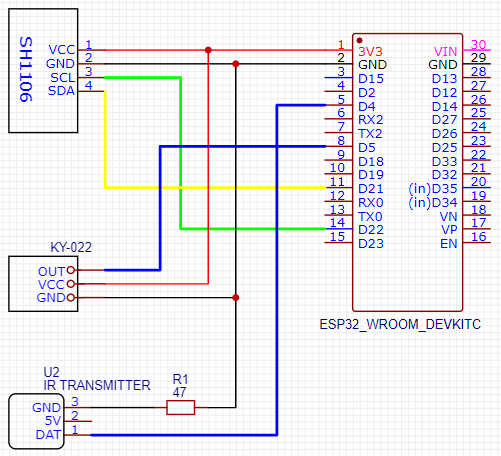
\includegraphics[width=12cm]{images/deviceScheme.png}
   \caption{Schemat elektryczny urządzenia pośredniczącego}
   \label{Fig:deviceScheme}
\end{figure}

Na schemacie kolorem czarnym oznaczono połączenia do GND, kolorem czerownym zasilanie z mikrokontrolera o potencjale 3.3V, na niebiesko zaznaczone są szyny danych modułów IR, a kolorami zielonym linię zegarową I2C oraz żółtym linię danych I2C wyświetlacza OLED.

Samo urządznie nie jest wrażliwe na zakłócenia elektromagnetyczne, ani nie wymagało stablinej obudowy do przestestowania poprawności założeń projektowych oraz końcowych testów pełnego systemu, dlatego jako element łączący moduły została użyta płytka stykowa. Dzięki użyciu płytki zachowano pełną funkcjonalność urządzenia oraz zyskano dowolność zmian podczas projektowania rozmieszczenia i połaczenia komponentów. Urządznie osadzone na płytce prototypowej zostało przedstawione na rysunku \ref*{Fig:deviceOnBoard}.
\begin{figure}[ht]
   \centering
   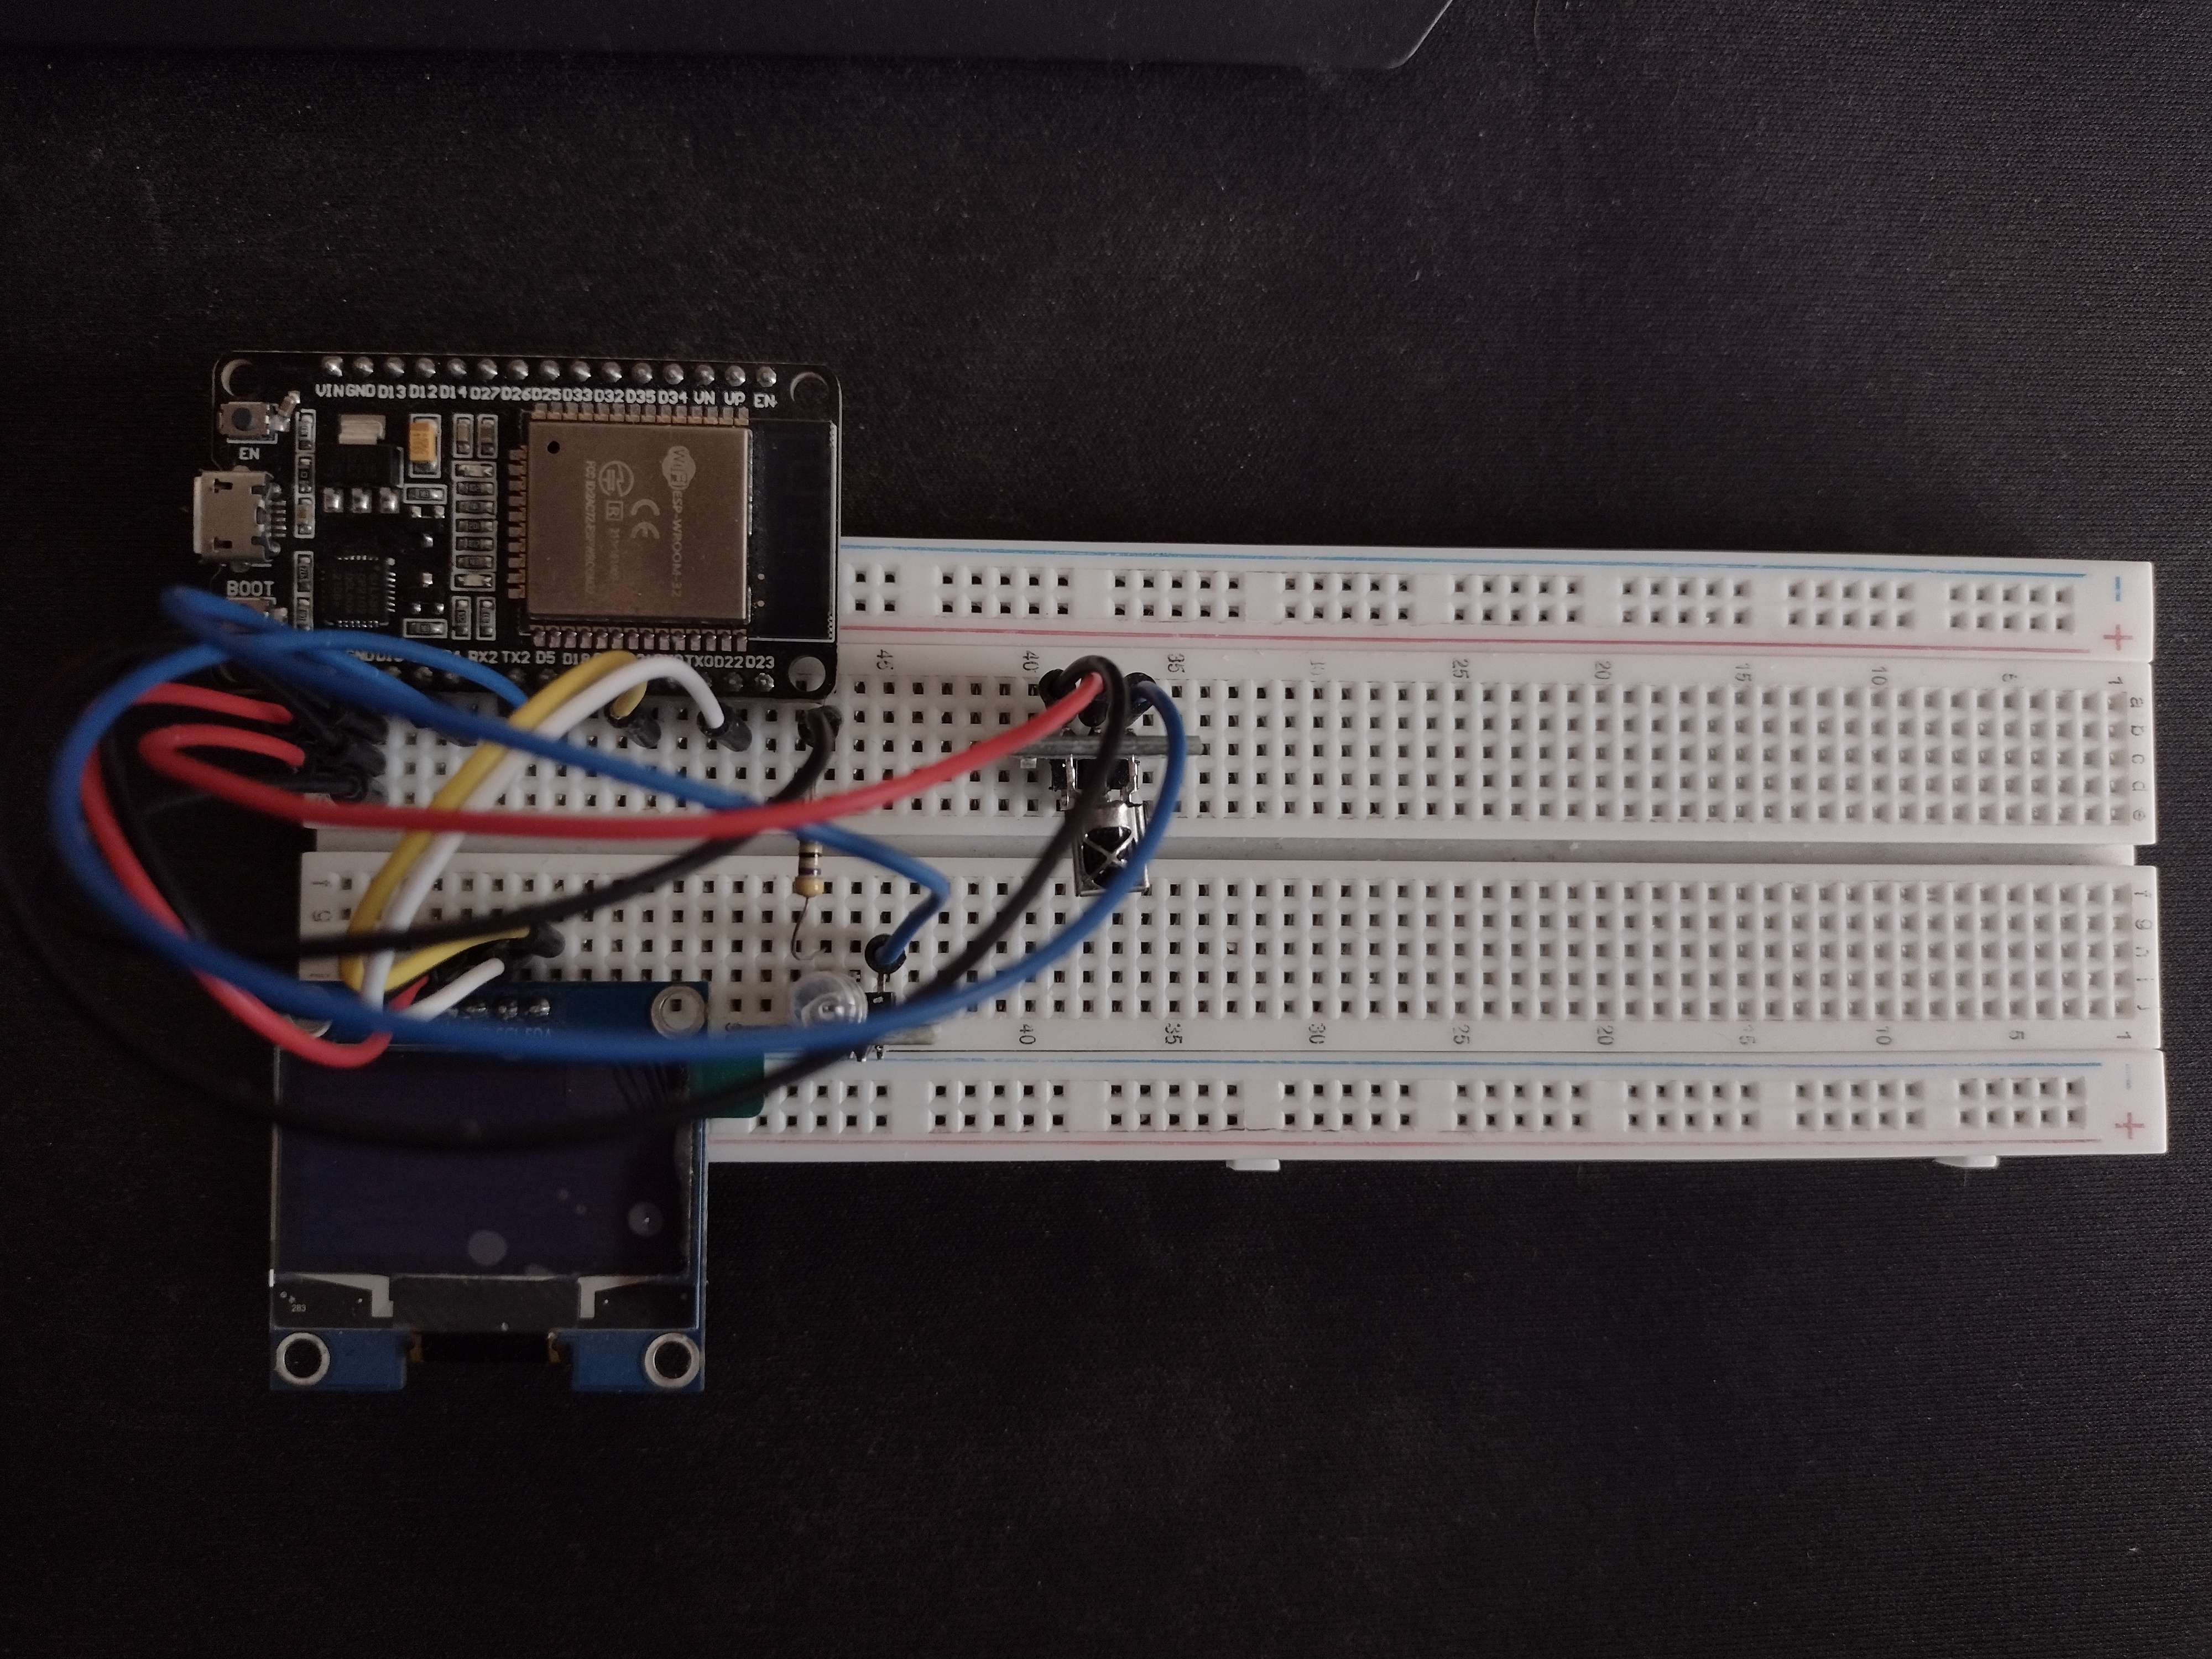
\includegraphics[width=12cm]{images/deviceOnBoard.jpg}
   \caption{Urządzenie pośredniczące osadzone na płytce prototypowej}
   \label{Fig:deviceOnBoard}
\end{figure}
\subsection{Przegląd i opis użytych komponentów}
Elementy przedstawione na schemacie elektrycznym znalazły się w przedstawionym wcześniej modelu modelu fizycznym. Są to:
\begin{enumerate}[label=\alph*), leftmargin=1.25cm]
   \item Płytka deweloperska ESP32 Wroom DevKitC V1\cite{doitDevKitV1} - to system z mikrokontroler ESP32 z procesorem Dual Core Tensilica LX6 240 MHz, pamięcią SRAM 520 KB i pamięcią flash 4 MB. Posiada wbudowane moduły WiFi 802.11 b/g/n oraz moduł Bluetooth Low Energy, dzięki którym nie trzeba dołączać osobnych modułów komunikacji bezprzewodowej. Znajduje się na nim 30 wyprowadzeń GPIO w postaci goldpinów, co znacznie zwiększa wygodę projektowania. Zasilany jest z 5 V ze złącza microUSB lub pinu VCC i GND.
   \item Wyświetlacz OLED SH1106\cite{sh1106}- to wyświetlacz OLED o przekątnej 1,3'' i rozdzielczości 128 pikseli na 64 pikesle. Ekran oparty jest na sterowniku Adafruit SH1106 pracuje z napięciami 3,3 V oraz 5 V, komunikuje się poprzez protokół I2C. Posiada wlutowane proste złącza goldpin. Wyświetla znaki w kolorze białym.
   \item Transmiter IR KY-005\cite{ky005} - to moduł nadawczy sygnałów podczerownych. Obsługuje wysyłanie fal IR o długości 940nm. I pobiera 90mW mocy podczas działania.
   \item Odbiornik IR KY-022\cite{ky022}  - to moduł z odbiorczy podczerwieni, działający na częstotliwości 38 kHz. Zasilany jest napięciem od 2,7 V do 5,5 V. Wykrywa sygnał pod maksymalnym kątem odchylenia 90°. Maksymalna odległość wykrywania: 18 m. Posiada cyfrowy sygnał wyjściowy.
   \item Rezystor 47 Ohm - resystor przewlekany o tolerancji 5\% i makasymalnej mocy 0,25 W.
   \item Przewody połaczeniowe męsko-męskie.
   \item Płytka stykowa.
\end{enumerate}

\clearpage

\section{Oprogramowanie sterujące urządzeniem wysyłającym sygnały IR}
\subsection{Środowisko narzędziowe}
Kod sterujący urządzeniem pośredniczącym opartym o mikrokontroler ESP32 został przygotowany za pomocą jezyka C++ oraz frameworka Arduino. Cały projekt oprogramowania zarządzany był przez rozszerzenie do edytora tekstu Visual Studio Code: PlatformIO, przy pomocy którego były doinstalowywane też wymagane biblioteki oraz budowany i wgrywany na płytkę ESP32 Wroom DevKitC program sterujący, a także przeprowadzane debugowanie. Każda z tych operacji mogła się odbyć dzięki wsparciu programowania i debugowania za pomocą portu microUSB, które posiadała płytka oraz rozszerzenie edytora tekstu.
\subsection{Ogólna struktura oprogramowania}
Oprogramowanie sterujące urządzeniem wysyłąjącym sygnały podczerowne zostało podzielone na 4 elementy. Główny z nich to plik main.cpp gdzie odbywa się sterowanie urządzeniem korzystając przy tym z pozostałych modułów. Utworzone zostały 3 moduły narzędziowe, aby główny kod stał się bardziej przejrzysty oraz modularny. Opdowiadają one za obsługę wyświetlacza OLED, komunikację BLE oraz interpretację danych pochodzących z charakterystyk BLE. Wynikowa struktura podziału autorskich elementów oprogramowania została przedstawiona na rysunku \ref*{Fig:codeStructure}.
\begin{figure}[ht]
   \centering
   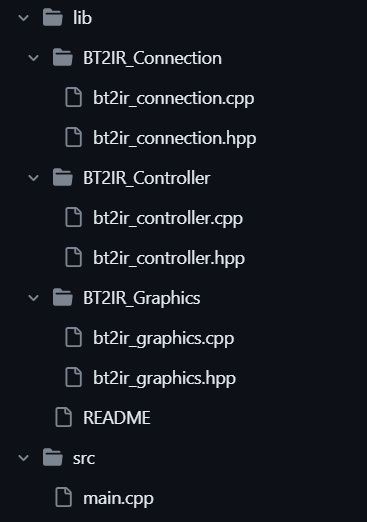
\includegraphics[width=4.5cm]{images/codeStructure.png}
   \caption{Struktura oprogramowania sterującego urządzeniem pośredniczącym}
   \label{Fig:codeStructure}
\end{figure}

\subsection{Główny program sterujący}
Główny program, który steruje urządzeniem pośredniczącym znajduje się w pliku ,,main.cpp''. Aby zorzumieć jakie funkcjonalności oferuje, najlepiej prześledzić jego budowę.

Najpierw dołączane są pliki nagłówkowe z framweworka Arduino dla ESP32 odpowiadające za obsługę wysyłu i odbioru syngałów podczerwonych. Dołączane są także autorskie moduły, które można poznać po przedrostku ,,bt2ir\_''. Korzystając z nich z kolei można utworzyć globalne obiekty klas, które pozwalają na zarządzanie połączeniem BLE,interpretacje danych z charakterystyk tego połączenia, i pracę z  wyświetlaczem OLED. Obiekty tych klas zostają zinicjowane odpowiednimi danymi prawidłowymi dla posiadanego sprzętu jak rozdzielczość ekranu OLED czy numery pinów płytki deweloperskiej, na których będą przesyłane dane z i do modułów IR. Prametry zostały opatrzone opisami za pomocą deyrektyw \#define oraz stałych aby zwiększyć czytelność ich przekazywania do konstruktorów. Kod realizujący dołączanie plików nagłówkowych oraz inicjalizację obiektów globalnych znajduje się na List.\ref{Lst:globalDefinitions}.

\lstinputlisting[inputencoding=utf8/cp1250, language={C++}, caption={\protect\input{captions/globalDefinitions.txt}\protect\relax}, label={Lst:globalDefinitions}]{codes/globalDefinitions.cpp}

Framework Arduino oczekuje zedefiniowania funkcji setup(), która będzie wykonywana raz podczas uruchomienia urządzenia. Utworzono takową i zawarto w niej już na początku zainicjowanie połaczenia szeregowego, aby móc odebrać dane z urządzenia na wypadek chęci wykrycia błędów działania. Znalazła się tam też inicjacja połaczenia z wyświetlaczem OLED poprzez protokół I2C i inicjacja serwera BLE, oba inicjacie zostały przeprowadzone za pomocą metod obiektów klas z autorskich modułów. Rozpoczęto w tej funkcji także nasłuchiwanie sygnałów podczerwonych i zainicjowano pracę modułu wysyłającego sygnały IR przy pomocy wcześniej utworzonych obiektów. Zawartość funkcji setup() przedstawia kod źródłówy na listingu List.\ref*{Lst:setup}.

\lstinputlisting[inputencoding=utf8/cp1250, language={C++}, caption={\protect\input{captions/setup.txt}\protect\relax}, label={Lst:setup}]{codes/setup.cpp}

Tworząc oprogramowanie za pomocą frameworka Arduino zdefiniować należy także funkcję, która będzie wykonywana w nieskończonej pętli na programowanym urządzeniu. Narzędzie wymaga nazywała się ona loop(). Przed nią jednak znalazły się jeszcze inicjalizacje dwóch znaczników czasowych w postaci dodatnich liczb całkowitych, które zostaną użyte do odliczania czasu trwania wyświetlania komunikatów dla użytkownika. 

W samej już funkcji umieszczono instrukcje warunkowe, przez które, sprawdzane jest czy wstąpiły zdarzenia takie jak: odebranie danych o wciśniętym klawiszu w aplikacji za pomocą serwera BLE, odebranie sygnału podczerwonego na module odbiornika IR, czy też rozłączenie lub połączenie z serwerem BLE nowego użytkownika aplikacji mobilnej. Jeśli funkcja wykryje zdarzenie serwera BLE, rysuje na wyświetlaczu OLED odświeżony aktualny stan połaczenia zwierający informację o liczbie połączonych użytkowników. Jeśli z kolei wykryte zostanie zdarzenie odebrania na serwerze BLE informacji o typie wciśniętego przycisku, rysowana jest jego ikona i nazwa aby poinformować użytkownika o odebraniu jego żądania. Po obsłużeniu zdarzenia resetowana jest flaga informująca o jego aktywności. Obsługa opisanych zdarzeń w pierwszej części funkcji loop() została przedstawiona na List.\ref*{Lst:loop1}.
\lstinputlisting[inputencoding=utf8/cp1250, language={C++}, caption={\protect\input{captions/loop1.txt}\protect\relax}, label={Lst:loop1}]{codes/loop1.cpp}

Program reaguje też na otrzymanie szesnastkowego kodu IR po wciśnieciu przycisku na pilocie w aplikacji. Po otrzymaniu tego kodu przez BLE przesyłany jest on dalej w formie sygnału podczerwonego do telewizora, realizując w ten sposób sterowanie nim i po zakończeniu obsługi zdarzenia resetowany jest jego flaga. Jeżeli odczytany zostanie, na zewnętrznym module odbiorczym, prawidłowy sygnał podczerwony, wypisany zostaje on na wyświetlaczu OLED, dzięki dedykowanej metodzie obiektu sterującego tym ekranem. Aktualizowany zostaje też wtedy znacznik czasowy tego zdarzenia. Następnie też wznawiane jest nasłuchiwanie sygnałów podczerwonych w tym module. Każdy z komunikatów dla użytkownika posiada swój czas wyświetlania. Limitowanie czasu ich trwania jest realizowane za pomocą sprawdzania stempli czasowych. Jeśli któryś z komunikatów powinien już się zakończyć, co jest wnioskowane na podstawie odległości aktualnego czasu od odpowiedniego znacznika czasowego, resetowane są wszystkie znaczniki czasowe komunikatów i następuje wyświetlenie domyślnego ekranu stanu połączenia BLE. Te funkcjonalności znalazły się w drugiej części funkcji loop(), a jej kod źródłowy został przedstawiony na List.\ref{Lst:loop2}.
\lstinputlisting[inputencoding=utf8/cp1250, language={C++}, caption={\protect\input{captions/loop2.txt}\protect\relax}, label={Lst:loop2}]{codes/loop2.cpp}
\subsection{Moduł komunikacji przez BLE}
Autorski moduł odpowiedzialny za komunikację BLE został oparty o moduły biblioteki nimBLE, zamiast podstawowej biblioteki BLE przygotowanej przez Arduino, ponieważ ta druga zajmowała zbyt wiele pamięci i nie mieściła się w pamięci FLASH mikrokontrolera. Wszystkie elementy tego modułu znalazły się w przestrzeni nazw bt2ir.

Klasa zarządzająca połaczeniem BLE została utworzona przy pomocy wzorca projektowego Singleton\cite{designPatterns}, który zapewnia utworzenie tylko jednej instancji takiej klasy. Zasosowano ten wzorzec aby zachowywać informacje o połączeniu BLE w całym programie. Publicznie funkcjonalności tej klasy udostępnione za pomocą metod to:
\begin{enumerate}[label=\alph*), leftmargin=1.25cm]
   \item inicjalizacja serwera BLE
   \item możliwość odczytywania i edytowania licznika połączonych urządzeń
   \item możliwość odczytywania i edytowania flag zdarzeń odebrania danych wciśniętego przycisku w aplikacji mobilnej
   \item dostęp do charakterystyk odebranego typu przycisku i jego kodu IR 
   \item metoda pozwalająca narysować aktualny stan połączenia BLE.
\end{enumerate} Część pliku nagłówkowego zawierająca dostępne metody publiczne klasy Connection została przedstawiona na List.\ref*{Lst:bleMethods}.

\lstinputlisting[inputencoding=utf8/cp1250, language={C++}, caption={\protect\input{captions/bleMethods.txt}\protect\relax}, label={Lst:bleMethods}]{codes/bleMethods.cpp}

Najważniejszym elementem tego modułu jest metoda setupConnection() klasy Connection. W niej właśnie odbywa się inicjowanie serwera BLE wraz z jego parametrami oraz dołączenie funkcji wywoływanych podczas zdarzeń serwera.

Podczas przygotowywania urządzenia pośredniczącego do obsługi BLE w pierwszej kolejności inicjowane jest urządzenie BLE. Kolejno dalej na urządzeniu tworzony jest serwer i przypisywane są mu autorskie klasy przechowujące callbacki zdarzeń serwera, zawarte także w tym module, dzięki czemu biblioteka automatycznie będzie wykonywać czynności po połączeniu i rozłączeniu użytkownika, oraz o takim wydarzeniu zostanie poinformowany główny program sterujący. 
Na tak utworzonym serwerze tworzony jest serwis i 2 jego charakterystyki odpowiadające wyłącznie za odbieranie danych o typie wciśniętego przycisku i jego szesnastkowym kodzie IR. Obie charakterystyki otrzymują także swoje klasy z metodami wywoływanymi podczas odebrania danych, dzięki czemu główny program sterujący informowany jest o tym zdarzeniu. Utworzony w ten sposób serwer może rozpocząć rozgłaszanie swojej obecności i nazwiązywać połączenia z klientami. Kod funkcji realizującej inicjalizację serwera BLE znajduje się na List.\ref*{Lst:setupConnection}. 

\lstinputlisting[inputencoding=utf8/cp1250, language={C++}, caption={\protect\input{captions/setupConnection.txt}\protect\relax}, label={Lst:setupConnection}]{codes/setupConnection.cpp}

Aby uzyskać możliwość połaczenia wielu użytkowników z serwerem urządzenia pośredniczącego metoda wywoływana podczas każdego połączenia nowego użytkownika musi wznowić rozgłaszanie dostępności serwera.
\subsection{Moduł interpretujący dane z BLE}
Aby ułatwić pracę z danymi odebranymi przez urządznie pośredniczące utworzono moduł przetwarzający te dane. Zawiera on wygodny enumerator wykorzystywany do nadania przejrzystych nazwy programowych dla odebranych typów wciśniętego przycisku pilota aplikacji mobilnej.
Z kolei klasa Controller odpowiada za interpretację danych odebranych za pomocą charakterystyk serwera BLE. Korzysta z ona z instancji klasy Connection aby pobrać dane charakterystyk i je zinterpretować. Udostępnia metody pozwalające odświeżać przechowywane w polach tej klasy ostatnio odebrane dane od aplikacji mobilnej.


\subsection{Biblioteka obsługi ekranu OLED}
Opis autorskiego modułu-nakładki do wyświetlania elementów na ekranie OLED węgiel.
\clearpage

\section{Aplikacja sterująca telewizorem}
\subsection{Struktura aplikacji}
Przedstawienie ogólnego zamysłu aplikacji i podziału na ekrany.
\subsection{Moduł obsługujący BLE}
Opis modułu odpowiedzialnego za komunikację BLE.
\subsection{Ekran połączenia z urządzeniem wysyłającym sygnał IR}
Przedstawienie funkcjonalności ekranu i przyjętych rozwiązań.
\subsection{Moduł obsługi przechowywania modelu telewizora}
Przedstawienie tego modułu.
\subsection{Ekran wyboru i edycji modelu telewizora}
Przedstawienie funkcjonalności ekranu i przyjętych rozwiązań.
\subsection{Ekrany przycisków pilota}
Przedstawienie funkcjonalności ekranu i przyjętych rozwiązań.
\clearpage

\section{Testy i prezentacja finalnego systemu}
W każdym z rozdziałów ewentualne wady rozwiązania i komentarze.
\subsection{Ustanawianie połączenia aplikacji z urządzeniem}
Przedstawienie sposobu nawziązywania połączenia aplikacji mobilnej z mikrokontrolerem.
\subsection{Edycja i wybór modelu telewizora w aplikacji}
Przedstawienie dostępnych opcji dodania, usunięcia i edycji czy wyboru modelu telewizora w którym znajdują się przyciski z kodami IR.
\subsection{Korzystanie z przycisków pilota}
Prezentacja działania systemu w kontakcie z telewizorem.

\clearpage

\section{Zakończenie}

1 $\div$ 3 stron merytorycznie podsumowanie najważniejszych elementów pracy oraz wnioski wynikające z osiągniętego celu pracy. Proponowane zalecenia i modyfikacje oraz rozwiązania będące wynikiem realizowanej pracy.

Ostatni akapit podsumowania musi zawierać wykaz własnej pracy dyplomanta i zaczynać się od sformułowania: „Autor za własny wkład pracy uważa: \ldots”.

\clearpage

\section*{Załączniki}
\addcontentsline{toc}{section}{Załączniki}

Według potrzeb zawarte i uporządkowane uzupełnienie pracy o dowolny materiał źródłowy (wydruk programu komputerowego, dokumentacja kons\-truk\-cyj\-no-\-tech\-no\-lo\-gicz\-na, konstrukcja modelu -- makiety -- urządzenia, instrukcja obsługi urządzenia lub stanowiska laboratoryjnego, zestawienie wyników pomiarów i obliczeń, informacyjne materiały katalogowe itp.).


\clearpage

\addcontentsline{toc}{section}{Literatura}
\bibliography{biblgr}
\bibliographystyle{plain}

\clearpage

\makesummary

\end{document}
